\documentclass[11pt]{article} 
\usepackage{amssymb, amsmath, amsthm}
\usepackage{tikz, graphicx, color, mathrsfs, rotating}
\usepackage{titlesec, lipsum}
\usepackage{fancyhdr, framed, chngcntr}

\usetikzlibrary{arrows,shapes,automata,backgrounds,decorations,petri,positioning,patterns}


\paperwidth = 8.5in
\paperheight = 11in
\textwidth = 6.5 in
\textheight = 9 in
\oddsidemargin = 0 in
\evensidemargin = 0 in
\topmargin = -.25 in
\headheight = 0.0 in
\headsep = .25 in
\footskip = .25in


\newtheorem*{repp@prob}{\repp@title}
\newcommand{\newreppprob}[2]{
\newenvironment{repp#1}[1]{
 \def\repp@title{#2 {##1}}
 \begin{repp@prob}}
 {\end{repp@prob}}}
\makeatother
\newreppprob{prob}{Problem}

\newtheorem*{repp@thm}{\repp@title}
\newcommand{\newreppthm}[2]{
\newenvironment{repp#1}[1]{
 \def\repp@title{#2 {##1}}
 \begin{repp@thm}}
 {\end{repp@thm}}}
\makeatother
\newreppthm{thm}{Theorem}


% -----------------------------------------------------------------------------
%             Macros for the course
% -----------------------------------------------------------------------------
\newcommand{\TS}{\mathcal{T}} % symbol for a topological space
\newcommand{\BS}{\mathcal{B}} % symbol for a basis
\newcommand{\R}{\mathbb{R}} % symbol for real numbers
\newcommand{\Z}{\mathbb{Z}} % symbol for integers
\newcommand{\Q}{\mathbb{Q}} % symbol for rational numbers
\newcommand{\PS}{\mathscr{P}} % symbol for power set
\newcommand{\E}{\mathbf{E}} % symbol for real numbers with Euclidean topology
\newcommand{\F}{\mathbf{F}^1} % symbol for real numbers with finite-complement topology
\renewcommand{\H}{\mathbf{H}^1} % symbol for real numbers with half-open topology
\renewcommand{\S}{\mathcal{S}} % basis topology
\newcommand{\B}{\mathbf{B}} % symbol for ball
\newcommand{\Sp}{\mathbf{S}} % symbol for sphere
\renewcommand{\int}{\operatorname{int}} % symbol for interior
\newcommand{\bnd}{\partial} % symbol for boundary
\newcommand{\homeo}{\approx} % symbol for homeomorphic


\begin{document} 


% -----------------------------------------------------------------------------
%             Start here
% -----------------------------------------------------------------------------

{\large
\noindent School of Computing %% replace "date" by the date on which the assignment was made
\hfill Chansu Park %% replace "Name" by your name

\vspace{.1in}

\noindent \today \hfill 20173245}

\vspace{.25in}

% -----------------------------------------------------------------------------
%             Erase or rearrange the options below, as necessary
% -----------------------------------------------------------------------------
\Large{
\begin{center}
\textbf{CS580}

Spring 2018, Homework \#1
\end{center}
}

\large

% -----------------------------------------------------------------------------
%             Template for typing up an Exercise
% -----------------------------------------------------------------------------
Here is the sample image that I made:
\begin{figure}[htb]
	\begin{center}
		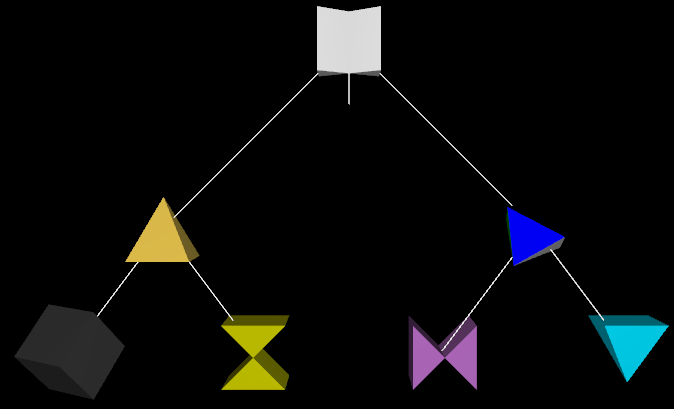
\includegraphics[width=0.6\linewidth]{mobile.png}
	\end{center}
	\caption{A sample mobile.}
\end{figure}

\section{Define three geometric primitives} \label{sec:1}
I proposed three objects: knot, pyramid, and octahedron.
\subsection{Knot} \label{ssec:1.1}
Originally, I tend to make a M\"obius strip, but there were several problems:
\begin{itemize}
	\item [i)] A little bit complex to translate the real one to the graphics;
	\item [ii)] A butterfly-shaped one (like Visual Studio logos) was quite complex;
	\item [iii)] According to our rendering method, if the orientation of vertices are reverted, then it cannot be rendered. In reality, only the front half can be rendered in the screen, whereas since M\"obius strip has an empty space, we can actually see the rear part, whereas computer graphics won't render.
\end{itemize}
Thus I generated a filled one:
\newpage
\begin{figure}[htb]
	\begin{center}
		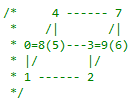
\includegraphics[width=0.3\linewidth]{knot.png}
	\end{center}
	\caption{A knot.}
\end{figure}
Surfaces $\{0, 1, 2, 3\}, \{3, 9, 2\}, \{9, 6, 7\}, \{8, 0, 3, 9\}, \{4, 8, 9, 7\}$ are visible; \\ surfaces $\{5, 4, 7, 6\}, \{4, 5, 8\}, \{8, 1, 0\}, \{9, 8, 5, 6\}, \{ 9, 2, 1, 8\}$ are not. \\ According to that I defined the correct order of vertices.

\subsection{Pyramid} \label{ssec:1.2}
\begin{figure}[htb]
	\begin{center}
		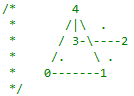
\includegraphics[width=0.3\linewidth]{pyramid.png}
	\end{center}
	\caption{A pyramid.}
\end{figure}

\subsection{Octahedron} \label{ssec:1.3}
Someone can make octahedron by attaching two pyramids with its square, but I didn't.
\begin{figure}[htb]
	\begin{center}
		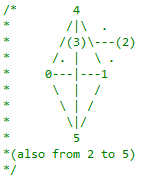
\includegraphics[width=0.2\linewidth]{octa.png}
	\end{center}
	\caption{An octahedron.}
\end{figure}

\section{Affine Transform Factorization} \label{sec:2}
\[
\left(\begin{matrix}
	l_{11} & l_{12} & l_{13} & t_1 \\
	l_{21} & l_{22} & l_{23} & t_2 \\
	l_{31} & l_{32} & l_{33} & t_3 \\
	0 & 0 & 0 & 1
\end{matrix} \right) = \left( \begin{matrix}
1 & 0 & 0 & t_1 \\
0 & 1 & 0 & t_2 \\
0 & 0 & 1 & t_3 \\
0 & 0 & 0 & 1
\end{matrix} \right) \left( \begin{matrix}
l_{11} & l_{12} & l_{13} & 0 \\
l_{21} & l_{22} & l_{23} & 0 \\
l_{31} & l_{32} & l_{33} & 0 \\
0 & 0 & 0 & 1
\end{matrix} \right)
\]
where the left hand side is the composition of the rotation and translation, and the first matrix of the right hand side is translation; the second one is rotation. \\
Since glm is column based, we have to extract the first three columns for $\operatorname{get\_linear}$; extract the last column for $\operatorname{get\_translation}$.

\subsection{\texttt{get\_linear}} \label{ssec:2.1}

\begin{figure}[htb]
	\begin{center}
		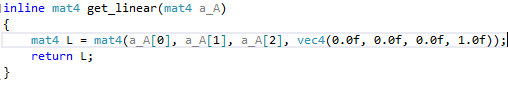
\includegraphics[width=0.8\linewidth]{getLinear.png}
	\end{center}
	\caption{We can construct a \texttt{mat4} type instance using 4 \texttt{vec4} type instance.}
\end{figure}

\subsection{\texttt{get\_translation}} \label{ssec:2.2}

\begin{figure}[htb]
	\begin{center}
		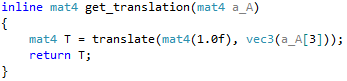
\includegraphics[width=0.8\linewidth]{getTrans.png}
	\end{center}
	\caption{We can extract the first 3 elements from a \texttt{vec4} instance using \texttt{vec3} initializer.}
\end{figure}

\section{Define Hierarchical Frames} \label{sec:3}

For a baby mobile, binary tree is sufficient. \\
There are several methods to implement binary tree. In particular, I used a Complete Binary Tree which every level, except possibly the last, is completely filled, and all nodes are as far left as possible.
\newpage
\begin{figure}[htb]
	\begin{center}
		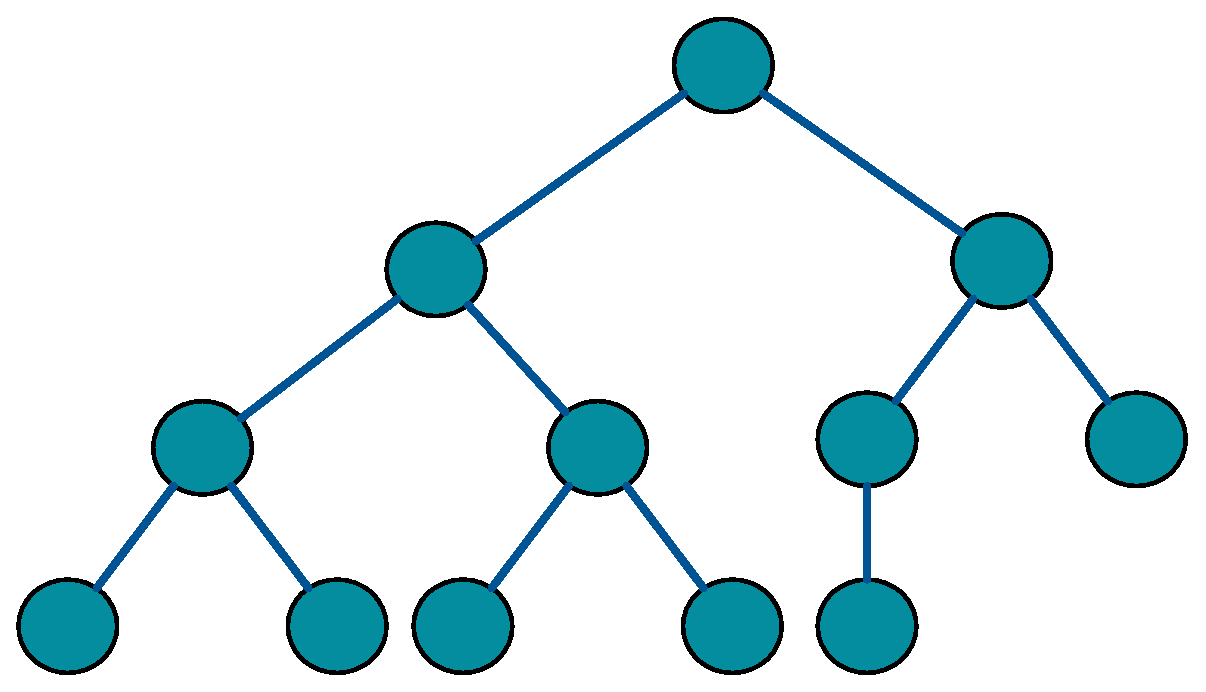
\includegraphics[width=0.5\linewidth]{CompleteBinary.eps}
	\end{center}
	\caption{An example of the complete binary tree.}
\end{figure}
Since we will place a node without any gap from the left nodes with the same level, we can give a number from 0 among nodes from root and from left to right. If a node has an index \texttt{i}, then we can find its children using indices \texttt{2i+1, 2i+2} if possible. It is just an array, so I implemented the tree using \texttt{c++ vector} with structure \texttt{ModelRbt}. It can be implemented without pointers.
\begin{figure}[htb]
	\begin{center}
		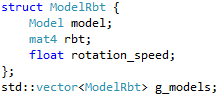
\includegraphics[width=0.4\linewidth]{gModel.png}
	\end{center}
	\caption{\texttt{g\_models[2i+1].rbt, g\_models[2i+2].rbt} will contain a relative transform from its parent \texttt{g\_models[i].rbt}.}
\end{figure}

Traversing this tree while applying rotation to the node is simple: process on the current node; go deep to childrens.

\section{Object Manipulation using Auxiliary Frame} \label{sec:4}

\section{Implementation for Keyboard Callbacks} \label{sec:5}

\section{Creativity} \label{sec:6}

%\begin{proof}[Solution.]
%% write your solution here
%\end{proof}


% -----------------------------------------------------------------------------
%             Template for typing up a Theorem
% -----------------------------------------------------------------------------
%\begin{reppthm}{42} %% replace "42" by the relevant Theorem number
%% restate the Theorem here
%\end{reppthm}

%\begin{proof}
%% write your proof here
%\end{proof}


% -----------------------------------------------------------------------------
%             End here
% -----------------------------------------------------------------------------

\end{document}